\documentclass{standalone}
\usepackage{tikz}
%------------tikz Setup------------

\tikzstyle{ball} = [circle,shading=ball, ball color=black,
    minimum size=1mm,inner sep=1.3pt]
\tikzstyle{miniball} = [circle,shading=ball, ball color=black,
    minimum size=1mm,inner sep=0.5pt]
\tikzstyle{mminiball} = [circle,shading=ball, ball color=black,
    minimum size=0.6mm,inner sep=0.1pt]
\usetikzlibrary{arrows.meta}
\usetikzlibrary{angles, quotes}
\tikzset{>={Latex[length=2mm,width=1.5mm]}}
\tikzset{->-/.style={decoration={markings, mark=at position #1 with
  {\arrow{>}}},postaction={decorate}}}
\usetikzlibrary{decorations.pathmorphing}
\usetikzlibrary{decorations.pathreplacing}
\usetikzlibrary{arrows.meta,calc}
\usetikzlibrary{bending}
\usetikzlibrary{decorations.markings,shapes.geometric}
\tikzset{->-/.style={decoration={markings, mark=at position #1 with
  {\arrow{>}}},postaction={decorate}}}
\tikzset{-|-/.style={decoration={markings, mark=at position #1 with
  {\arrow{stealth}}},postaction={decorate}}}
\tikzset{movearrow/.style 2 args ={
        decoration={markings,
    mark= at position {#1} with {\arrow{#2}} ,
        },
        postaction={decorate}
    }
}


\begin{document}
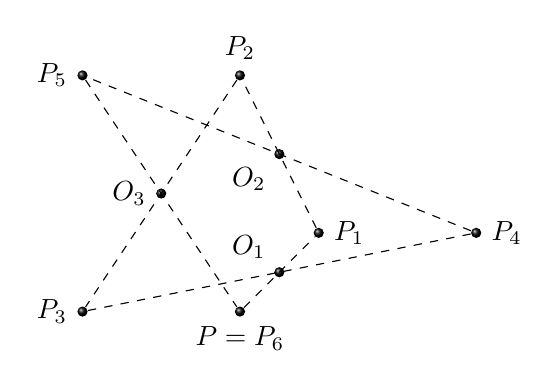
\begin{tikzpicture}
\begin{scope}[scale=0.5]
    %points
    \node[ball,label={below:$P=P_6$}] (p) at (0, -3) {};
    \node[ball,label={above left:$O_1$}] (o1) at (1, -2) {};
    \node[ball,label={below left:$O_2$}] (o2) at (1, 1) {};
    \node[ball,label={left:$O_3$}] (o3) at (-2, 0) {};
    \node[ball,label={right:$P_1$}] (p1) at (2, -1) {};
    \node[ball,label={above:$P_2$}] (p2) at (0, 3) {};
    \node[ball,label={left:$P_3$}] (p3) at (-4, -3) {};
    \node[ball,label={right:$P_4$}] (p4) at (6, -1) {};
    \node[ball,label={left:$P_5$}] (p5) at (-4, 3) {};
    %lines
    \draw[dashed] (p) to (p1);
    \draw[dashed] (p1) to (p2);
    \draw[dashed] (p2) to (p3);
    \draw[dashed] (p3) to (p4);
    \draw[dashed] (p4) to (p5);
    \draw[dashed] (p5) to (p);
\end{scope}
\end{tikzpicture}
\end{document}